\chapter{序論}
\thispagestyle{empty}
\label{Chap1}
\minitoc

\newpage
%%%%%%%%%%%%%%%%%%%%%%%%%%%%%%%%%%%%%%%%%%%%%%%%%%%%%%%%%%%%%%%%%%%%%%%%%%%%%%%

%==============================================================================
% 1.1
%==============================================================================
\section{背景}
\label{Demand}

新たなサービスの提供や作業の効率化を目的として,様々な分野においてロボットの導入が進んでいる.
ロボットの活用例として,工場や倉庫における無人搬送車の利用\mbox{\cite{ゾリーグ2014}}や,ドローンを用いたインフラ点検\mbox{\cite{Hada2017}}などが挙げられる.
このような作業をロボットに行わせるためには,ロボットの自己位置推定は必要不可欠な課題である.
特に,ドローンなどの空間を飛び回る移動ロボットを利用する際には,位置の3自由度と姿勢の3自由度,計6自由度の位置姿勢推定が必要となる.
\vspace{\baselineskip}

屋外環境において移動ロボットの自己位置推定を行う場合には,衛星からの電波を利用して位置を推定するシステムせある,Global Navigation Satellite System(GNSS)を用いることが一般的である\mbox{\cite{Ohno2004}}\mbox{\cite{Kim2007}}.
しかし,屋内環境では電波が届かないため利用することが難しい.
目印となる基準のマーカを用いて位置姿勢推定を行う研究\mbox{\cite{Olson2011}}も行われているが,環境にマーカを取り付ける必要があり,実用性に欠ける.
また,WiFiを用いる手法\mbox{\cite{Miyagusuku2016}}も提案されているが,WiFi環境の構築が必要であることや位置推定のみで姿勢は推定できない問題がある.
これらの手法に対し,ロボットにカメラを搭載して,カメラで取得する映像情報を用いて位置姿勢を推定する手法は,屋内環境においても利用でき,また環境に手を加えることなく推定が可能である.
\vspace{\baselineskip}

上記のように,GNSSが利用できない屋内環境におけるカメラの6自由度の位置姿勢推定は非常に重要である.
カメラの位置姿勢推定では,広範囲の視野を持つカメラを利用することが特に効果的である.
例えば,カメラが障害物に接近した場合に,通常の透視投影カメラでは障害物の一部であるごく狭い範囲の映像しか取得されず,位置姿勢推定に必要な情報を得ることができない.
このように,通常の透視投影カメラでは視野が制限されてしまう状況においても,広い視野を持つカメラであれば残りの範囲から情報を得ることができるため,よりロバストに位置姿勢推定を行うことが可能である.
\vspace{\baselineskip}

広い視野を持つカメラには,全方位カメラや全天球カメラと呼ばれる360 deg の視野を持つカメラがある.
全方位カメラは,双曲面ミラーに反射した物体を撮影することで半天球の視野を持つカメラである\mbox{\cite{八木2001}}\mbox{\cite{Panasonic}}\mbox{\cite{ELECOM}}\mbox{\cite{VSTONE}}.
通常の透視投影カメラと全方位カメラの視野の広さの違いを図~\ref{fig:OmniCam}に示す.
一方,全天球カメラとは,上下左右全方位の360 deg の広範囲の映像を一度に撮影できるカメラである\mbox{\cite{RICOH}}\mbox{\cite{Samsung}}\mbox{\cite{LG360}}.
全天球カメラは,魚眼カメラを両側に装備したり,Googleストリートビューの撮影装置のように3台以上のカメラを組み合わせたりすることによって,複数のカメラの視野を重ね合わせて360 deg の映像を生成するカメラである.
通常の透視投影カメラと全天球カメラの視野の広さの違いを図~\ref{fig:SphCam}に示す.
これらの図から確認できるように,全方位カメラや全天球カメラは通用の透視投影画像と比べて広範囲の映像を取得するため,位置姿勢推定のロバスト性の向上に有効である.
\vspace{\baselineskip}

\begin{figure}[b]
 \begin{center}
 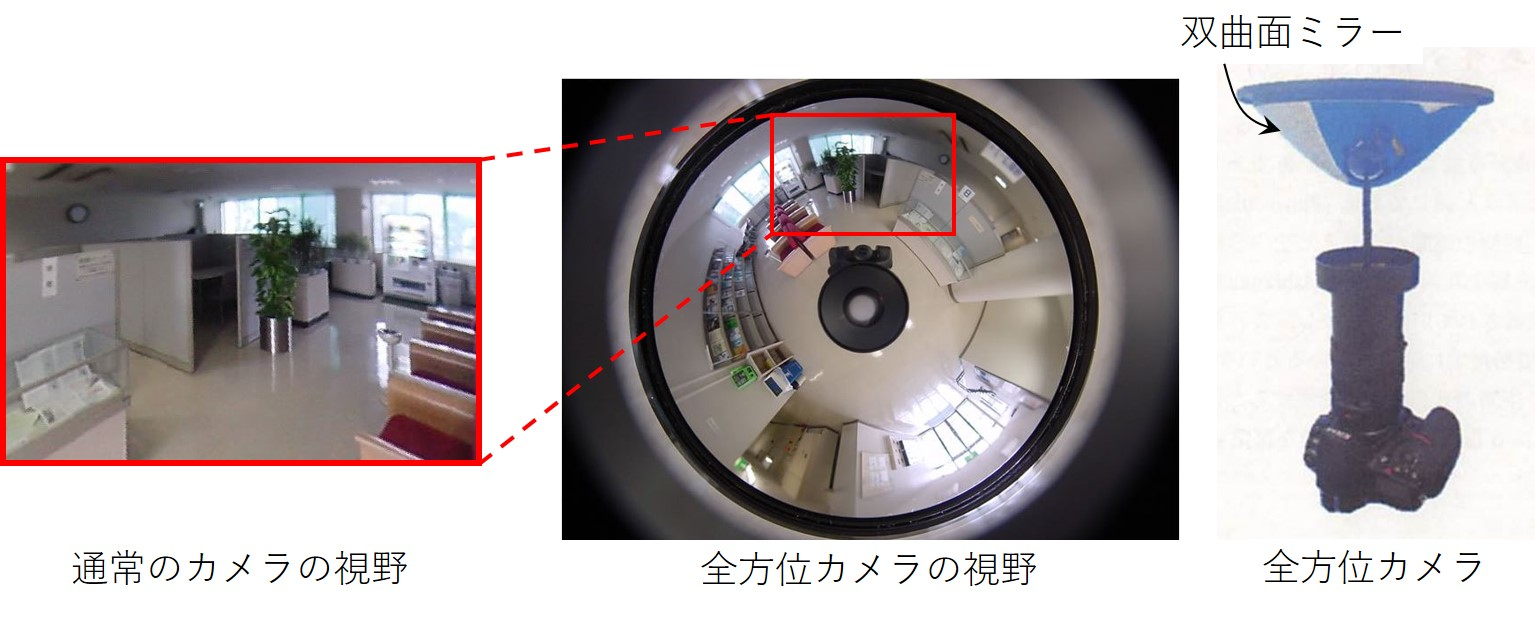
\includegraphics[width=0.9\columnwidth]{./chap1/fig/全方位.jpg}
 \caption{通常のカメラと全方位カメラの視野の比較}
 \label{fig:OmniCam}
 \end{center}
 \vspace{5mm}
\end{figure}

\begin{figure}[b]
 \begin{center}
 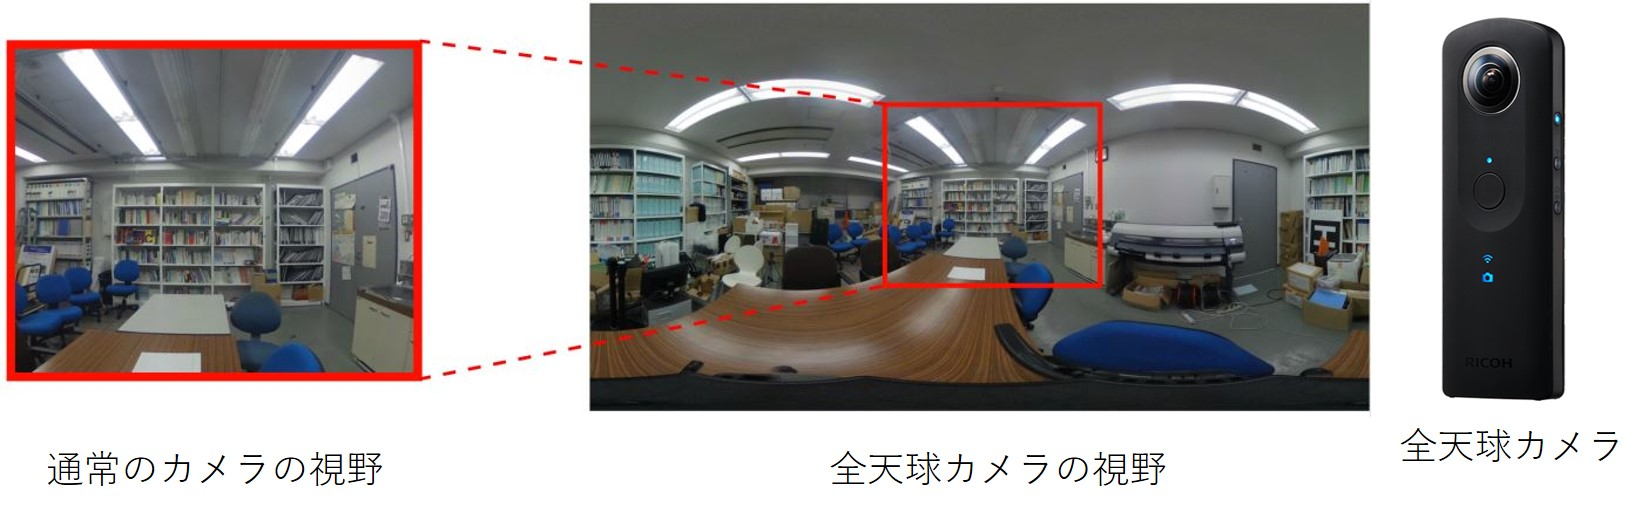
\includegraphics[width=0.9\columnwidth]{./chap1/fig/全天球.jpg}
 \caption{通常のカメラと全天球カメラの視野の比較}
 \label{fig:SphCam}
 \end{center}
 %\vspace{-5mm}
\end{figure}

\clearpage
%%==============================================================================
%% 1.2
%%==============================================================================
\section{カメラの位置姿勢推定に関する従来研究}
\label{Previous_study}

前節では,カメラを用いた6自由度の位置姿勢推定が重要であり,そのロバスト性の向上のためには全天球カメラのような,広い視野を持つカメラやが有効であることを述べた.
カメラの位置姿勢を推定する研究はこれまでにも数多く行われている.
本節では,それらの研究を位置姿勢推定のアプローチに関して分類してまとめる.
\vspace{\baselineskip}

画像から位置姿勢を推定する手法では,カメラの移動追跡を行う手法と,1枚の画像を用いて環境中から大域的に推定する手法がある.
カメラの移動追跡を行う手法では,Visual Odometry\mbox{\cite{Nister2004}}やSimultaneous Localization and Mapping(SLAM)\mbox{\cite{Klein2007}}\mbox{\cite{Caruso2015}}の研究があるが,カメラの移動量にともなって推定誤差が蓄積していく問題がある.
また,カメラの回転などの動きによって視野が大きく変わると追跡に失敗する場合がある\mbox{\cite{酒井2014}}.
このような場合など,新しく移動追跡を始めるためには,移動追跡の初期値を設定する必要があり,1枚の画像を用いて環境中から大域的に推定することが求められる.
そこで本研究では1枚の画像を用いて環境中から大域的に位置姿勢を推定する手法を構築する.
\vspace{\baselineskip}

環境中からの大域的な推定としては,環境のモデル等を参照情報として,取得した画像とマッチングすることで位置姿勢を推定する手法が一般的であり,これまでに数多く提案されている.
%環境の地図やモデルから任意の位置姿勢における環境中のシーンを再現することで,事前に大量の参照画像を用意する必要がないという利点がある.
これらの手法は,通常の透視投影カメラを用いた手法と全天球カメラを用いた手法の2つに大きく分けられる.
\\

はじめに,通常の透視投影カメラを用いた研究を示す.
%シーン中の物体のCADモデルを用いてカメラの位置姿勢を推定する手法が提案されている\mbox{\cite{Bleser2006}}\mbox{\cite{Aldoma2011}}.
%これらの研究では,CADモデルが既知の物体が画像中に写っていれば良いため,周りの環境の変化にロバストであるという利点がある.
%しかし,カメラの視野にCADモデルの物体をとらえている必要があるため,カメラの移動範囲が制限される問題点がある.
環境全体のモデルを用いた位置姿勢推定の研究として,都市環境で位置姿勢推定を行った研究がある\mbox{\cite{Sattler2011}}.
しかし,この研究では特徴点の位置合わせによって位置姿勢を推定しており,移動物体などのノイズの影響に弱い.
特徴点ベースではなく,画像とモデルの直線の対応から位置姿勢を推定する手法も提案されている\mbox{\cite{Mirzaei2011}}\mbox{\cite{Vakhitov2016}}\mbox{\cite{Xu2017}}.
しかし,これらの手法では直線の対応を事前に与える必要がある.
Jiら\mbox{\cite{Ji2017}}は,カメラ画像から抽出した直線特徴を用いて,壁に固定されたカメラのロバストな5自由度の位置姿勢推定を行っている.
しかし,この手法は通常の透視投影カメラのみに適用可能であり,全天球カメラ画像に対して適用することはできない.
%全天球カメラ画像では直線は歪んで描画されるため,全天球カメラのより広範囲の画像を効果的に利用するためには,この歪みを考慮した直線検出手法やマッチング手法が必要となる.
\\

次に,広い視野を持つカメラを用いた研究を示す.
事前に環境中のシーンの画像をメモリに保存しておき,メモリ中の画像を参照情報として,位置姿勢を推定したい画像とメモリ中の画像を比較することで全方位カメラの位置姿勢を推定する手法が提案されている\mbox{\cite{Aihara1998}}.しかし,この手法では参照する画像を大量に用意する必要があり,また大きなメモリを必要とする問題がある.
また,建物の隙間から見える空の形状を利用する研究\mbox{\cite{Ramalingam2011}}や,構造物のエッジや直線を利用した研究\mbox{\cite{Mariottini2007}}\mbox{\cite{Cham2010}}\mbox{\cite{Ishizuka2011}}\mbox{\cite{Caron2012}}が数多く提案されている.
しかし,これらの研究はすべて,平面内の3自由度の位置姿勢推定のみを行っており,空間の6自由度に拡張することは困難である.
Gotoら\mbox{\cite{Goto2018}}は,直線特徴に基づく3D-2Dマッチングを用いた全天球カメラの6自由度の位置姿勢推定手法を提案している.
しかし,この手法はオフラインアプリケーションを想定しており,推定に時間がかかるため,カメラの移動追跡に失敗した際に新しく初期値を設定する場合など,高速に推定することが求められるアプリケーションに適用することは難しい.
\\

ここまでで,参照情報を用いてカメラの位置姿勢を推定する研究について述べた.
1.1節で述べたようにロバストな位置姿勢推定のためには全天球カメラの利用が有効である一方,幅広く応用可能な手法のためには6自由度の高速な位置姿勢推定が求められる.
しかし,全天球カメラを用いた6自由度の位置姿勢を高速に推定可能な手法は未だ確立されていない.
これらを踏まえ,次節では本研究の目的を述べる.

\clearpage
%%==============================================================================
%% 1.3
%%==============================================================================
\section{研究の目的}
\label{Objective}

1.1節で,全天球カメラなど視野の広いカメラを位置姿勢推定に用いる優位性を述べた.
しかし,1.2節にて,全天球カメラの高速な6自由度の位置姿勢推定の手法は未だ確立されていないことを示した.
\\

そこで,本研究の目的を以下のように設定する.

\vspace{5pt}
\begin{itembox}[c]{目的}
\begin{center}
直線情報を用いた全天球カメラの高速な6自由度の位置姿勢推定
\end{center}
\end{itembox}
\vspace{5pt}

計算時間の要求仕様は,カメラの移動追跡の初期値の設定など,高速に推定することが求められる場合にも適用できる時間として,数秒オーダーの計算時間を設定する.
精度については,適用するアプリケーションにより要求仕様が異なるため,本研究では特に要求仕様を設定しない.
例えば,移動ロボットを用いて老朽化したインフラを点検するアプリケーションにおいては,作業箇所を大まかに推定した後にその周囲を詳細に点検するため,多少の誤差が含まれても問題なく点検を遂行することが可能である.

\clearpage
%%==============================================================================
%%本論文の構成
%%==============================================================================
\section{本論文の構成}
\label{Structure}

本論文は全6章から構成されている.本論文の構成を図\ref{fig:structure}に示す.

第1章では,本研究の背景と従来研究,目的について述べた.

第2章では,問題設定を明かにし、本研究におけるアプローチについて述べる.

第3章では,姿勢推定について述べる.

第4章では,位置推定について述べる.

第5章では,本提案手法の有効性を検証するために行った実験について述べる.

第6章では,本研究に関する結論と今後の展望を述べる.

\begin{figure}[b]
 \begin{center}
 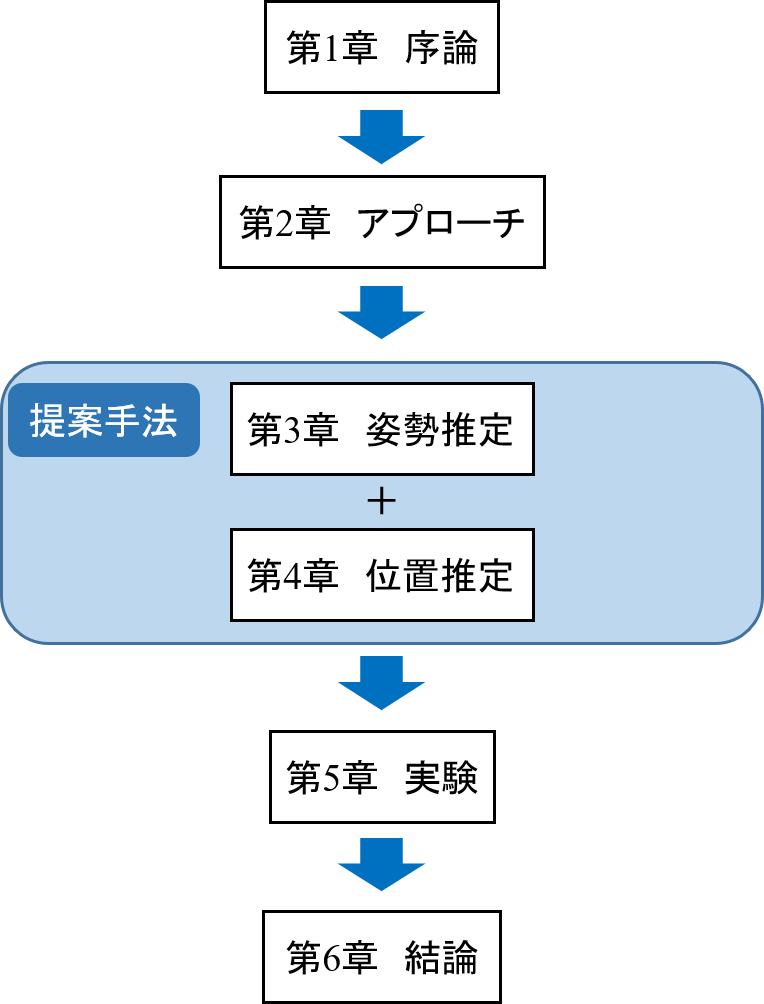
\includegraphics[width=0.50\columnwidth]{./chap1/fig/structure.png}
 \caption{本論文の構成}
 \label{fig:structure}
 \end{center}
\end{figure}

\clearpage
%%%%%%%%%%%%%%%%%%%%%%%%%%%%%%%%%%%%%%%%%%%%%%%%%%%%%%%%%%%%%%%%%%%%%%%%%%%%%%%
%%% Local Variables:
%%% mode: katex
%%% TeX-master: "../thesis"
%%% End: